\chapter{\label{method}Experimental Set-up}


%\begin{figure}
%	\centering
%	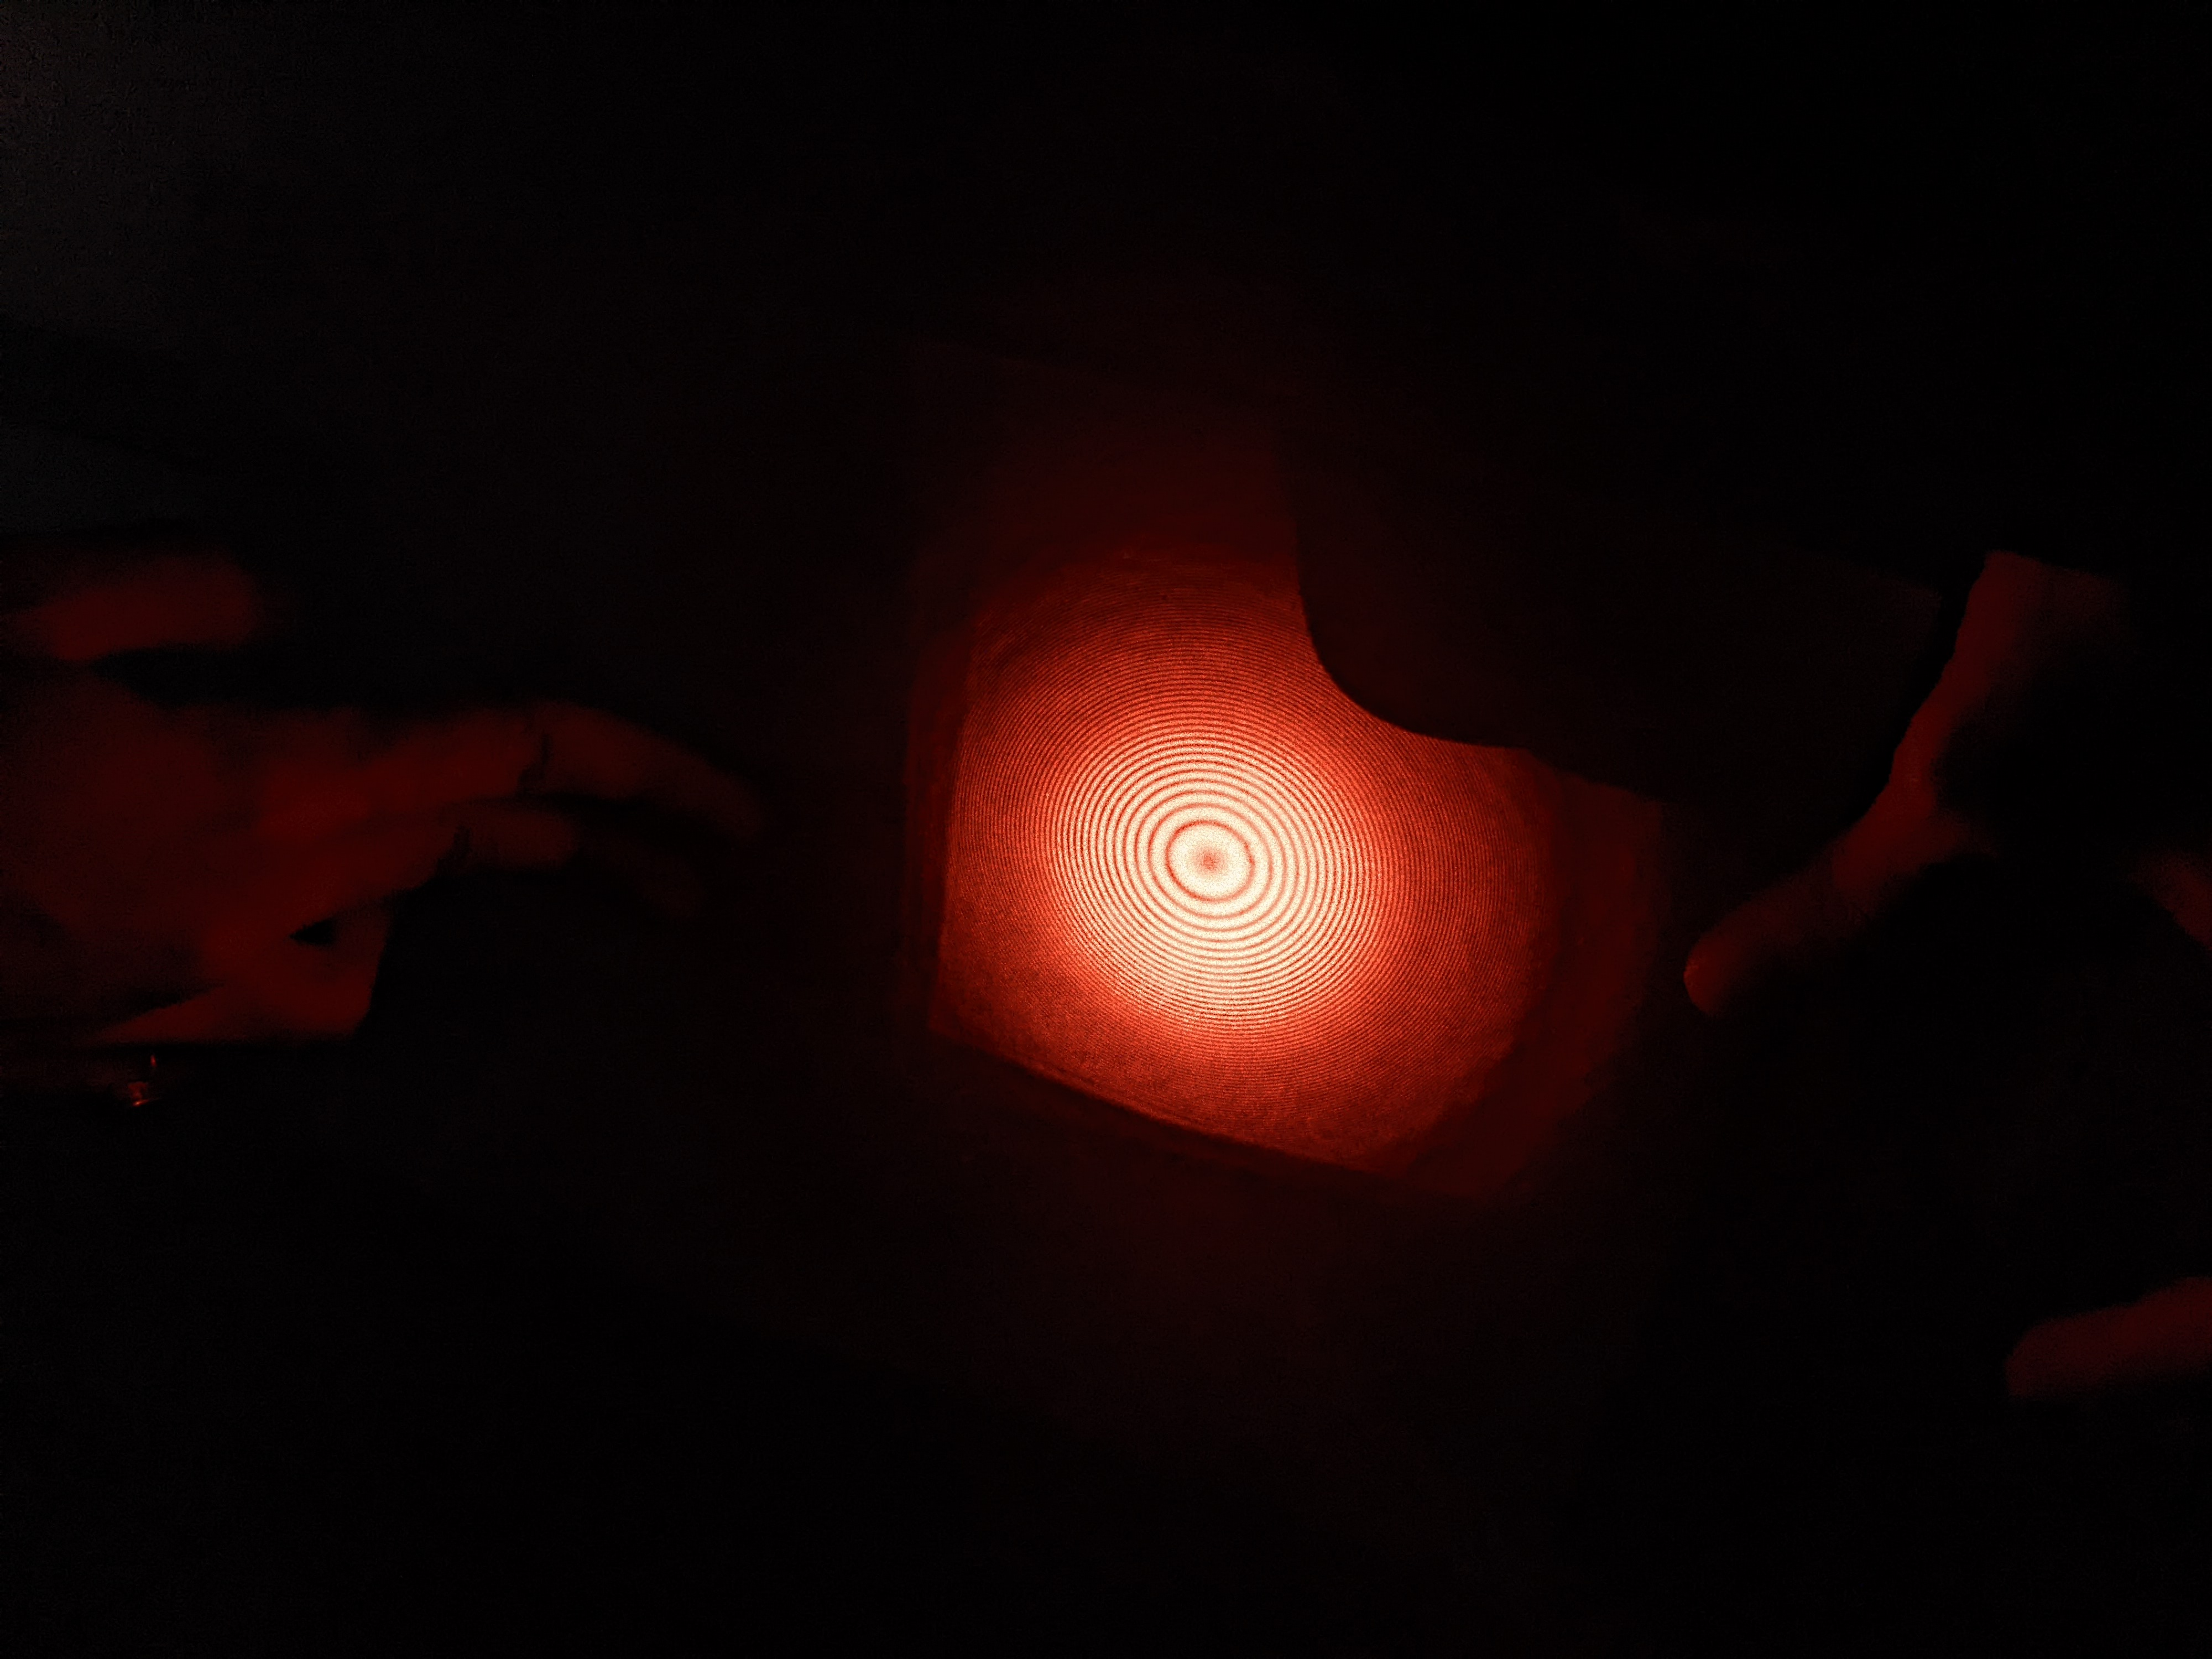
\includegraphics[width=0.7\linewidth]{SGCAM_20230117_144041192}
%	\caption{}
%	\label{fig:sgcam20230117144041192}
%\end{figure}
%\begin{figure}
%	\centering
%	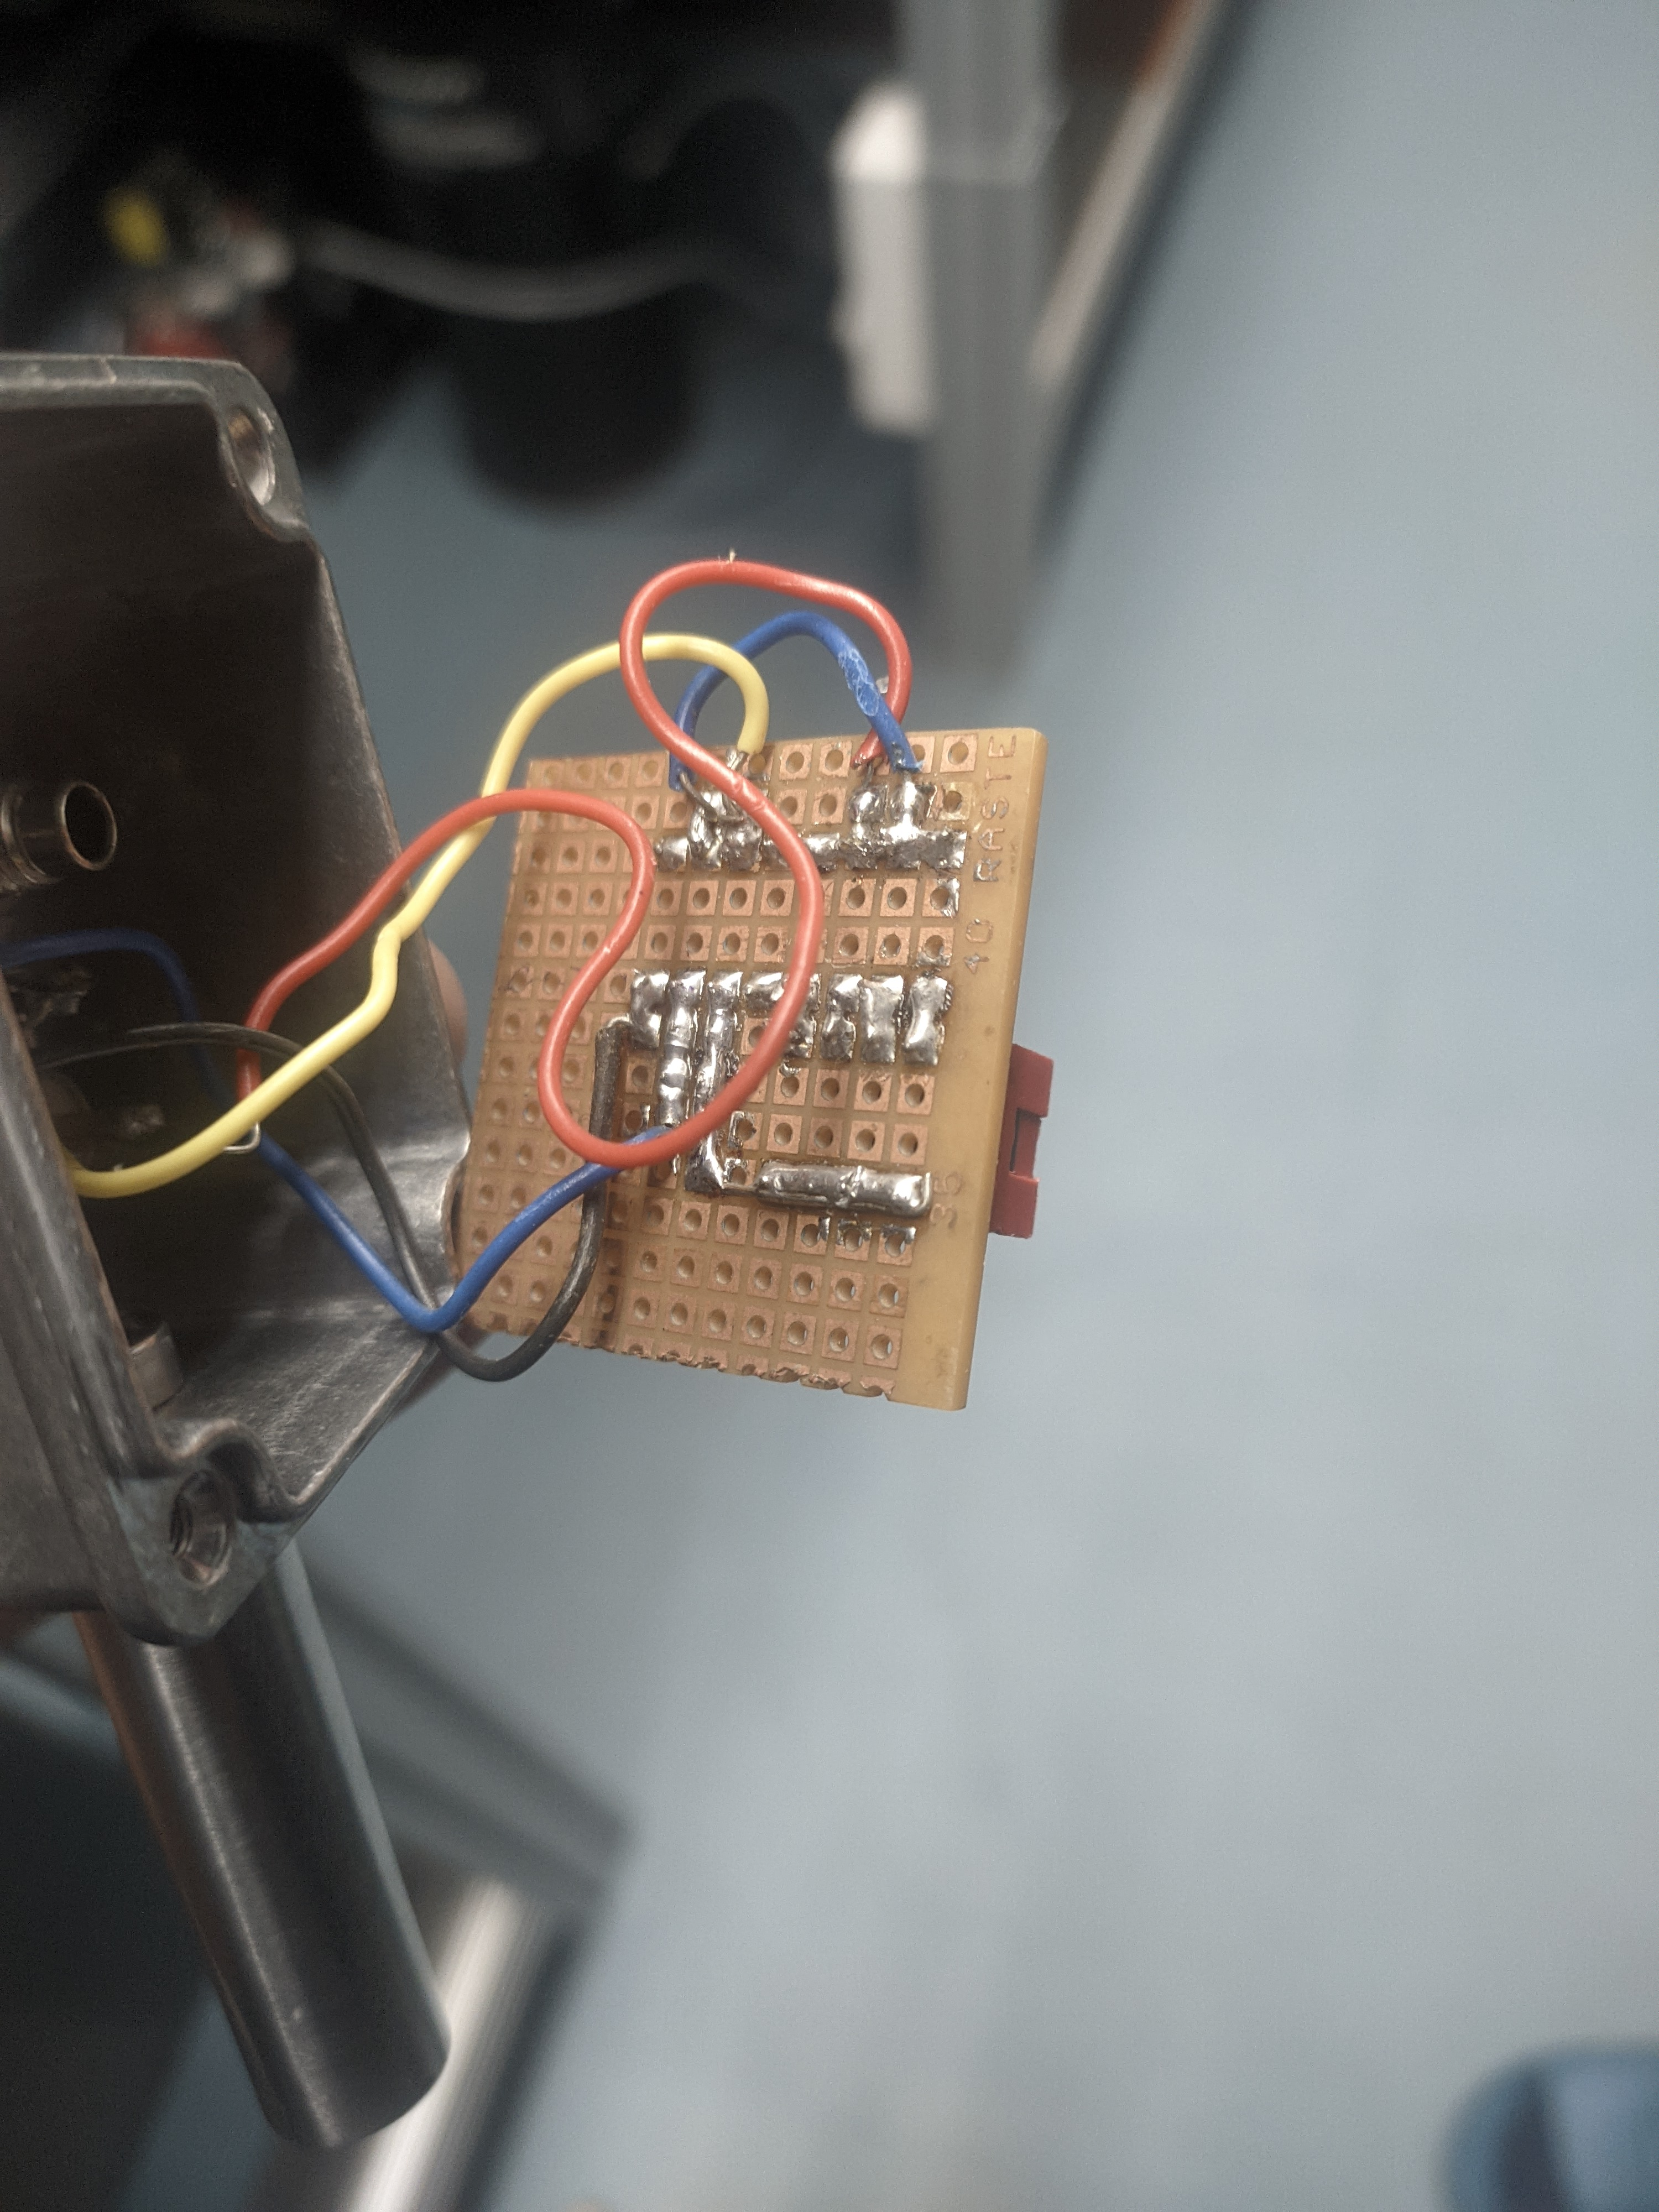
\includegraphics[width=0.7\linewidth]{SGCAM_20230110_170204378}
%	\caption{Photodetector circuitry}
%	\label{fig:sgcam20230110170204378}
%\end{figure}
\begin{figure}
	\centering
	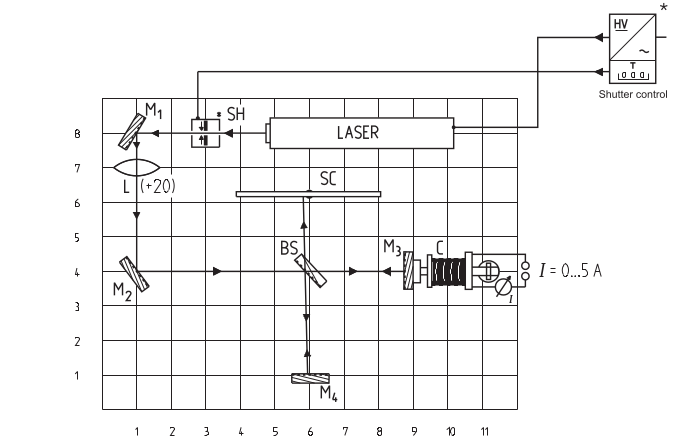
\includegraphics[width=0.7\linewidth]{schematic}
	\caption{Schematic of the experiment on the magnetic bench}
	\label{fig:schematic}
\end{figure}
The mirrors utilized in this setup are surface reflecting, which allows the incident beam to exit the mirror at the point of incidence. The laser beam is directed towards the first mirror M1 of the interferometer setup. Mirror M2 redirects the beam towards the beam splitter. The beam splitter transmits half of the radiation to the translatable mirror M3, while reflecting the other half towards the fixed mirror M4. After reflecting from M3, half of the light is directed towards the screen, and the other half from M4 is also transmitted to the screen. The rays from mirrors M3 and M4 interfere behind the glass plate, producing circular fringe patterns. In our experiment, we used a beam expander placed between M2 and the beam splitter to achieve this. When the length of one of the mirror arms changes, the interference pattern also changes, causing the collapse or generation of fringes. Figure 4 shows that the rod with the current coil is attached to mirror M3.

\begin{figure}
	\centering
	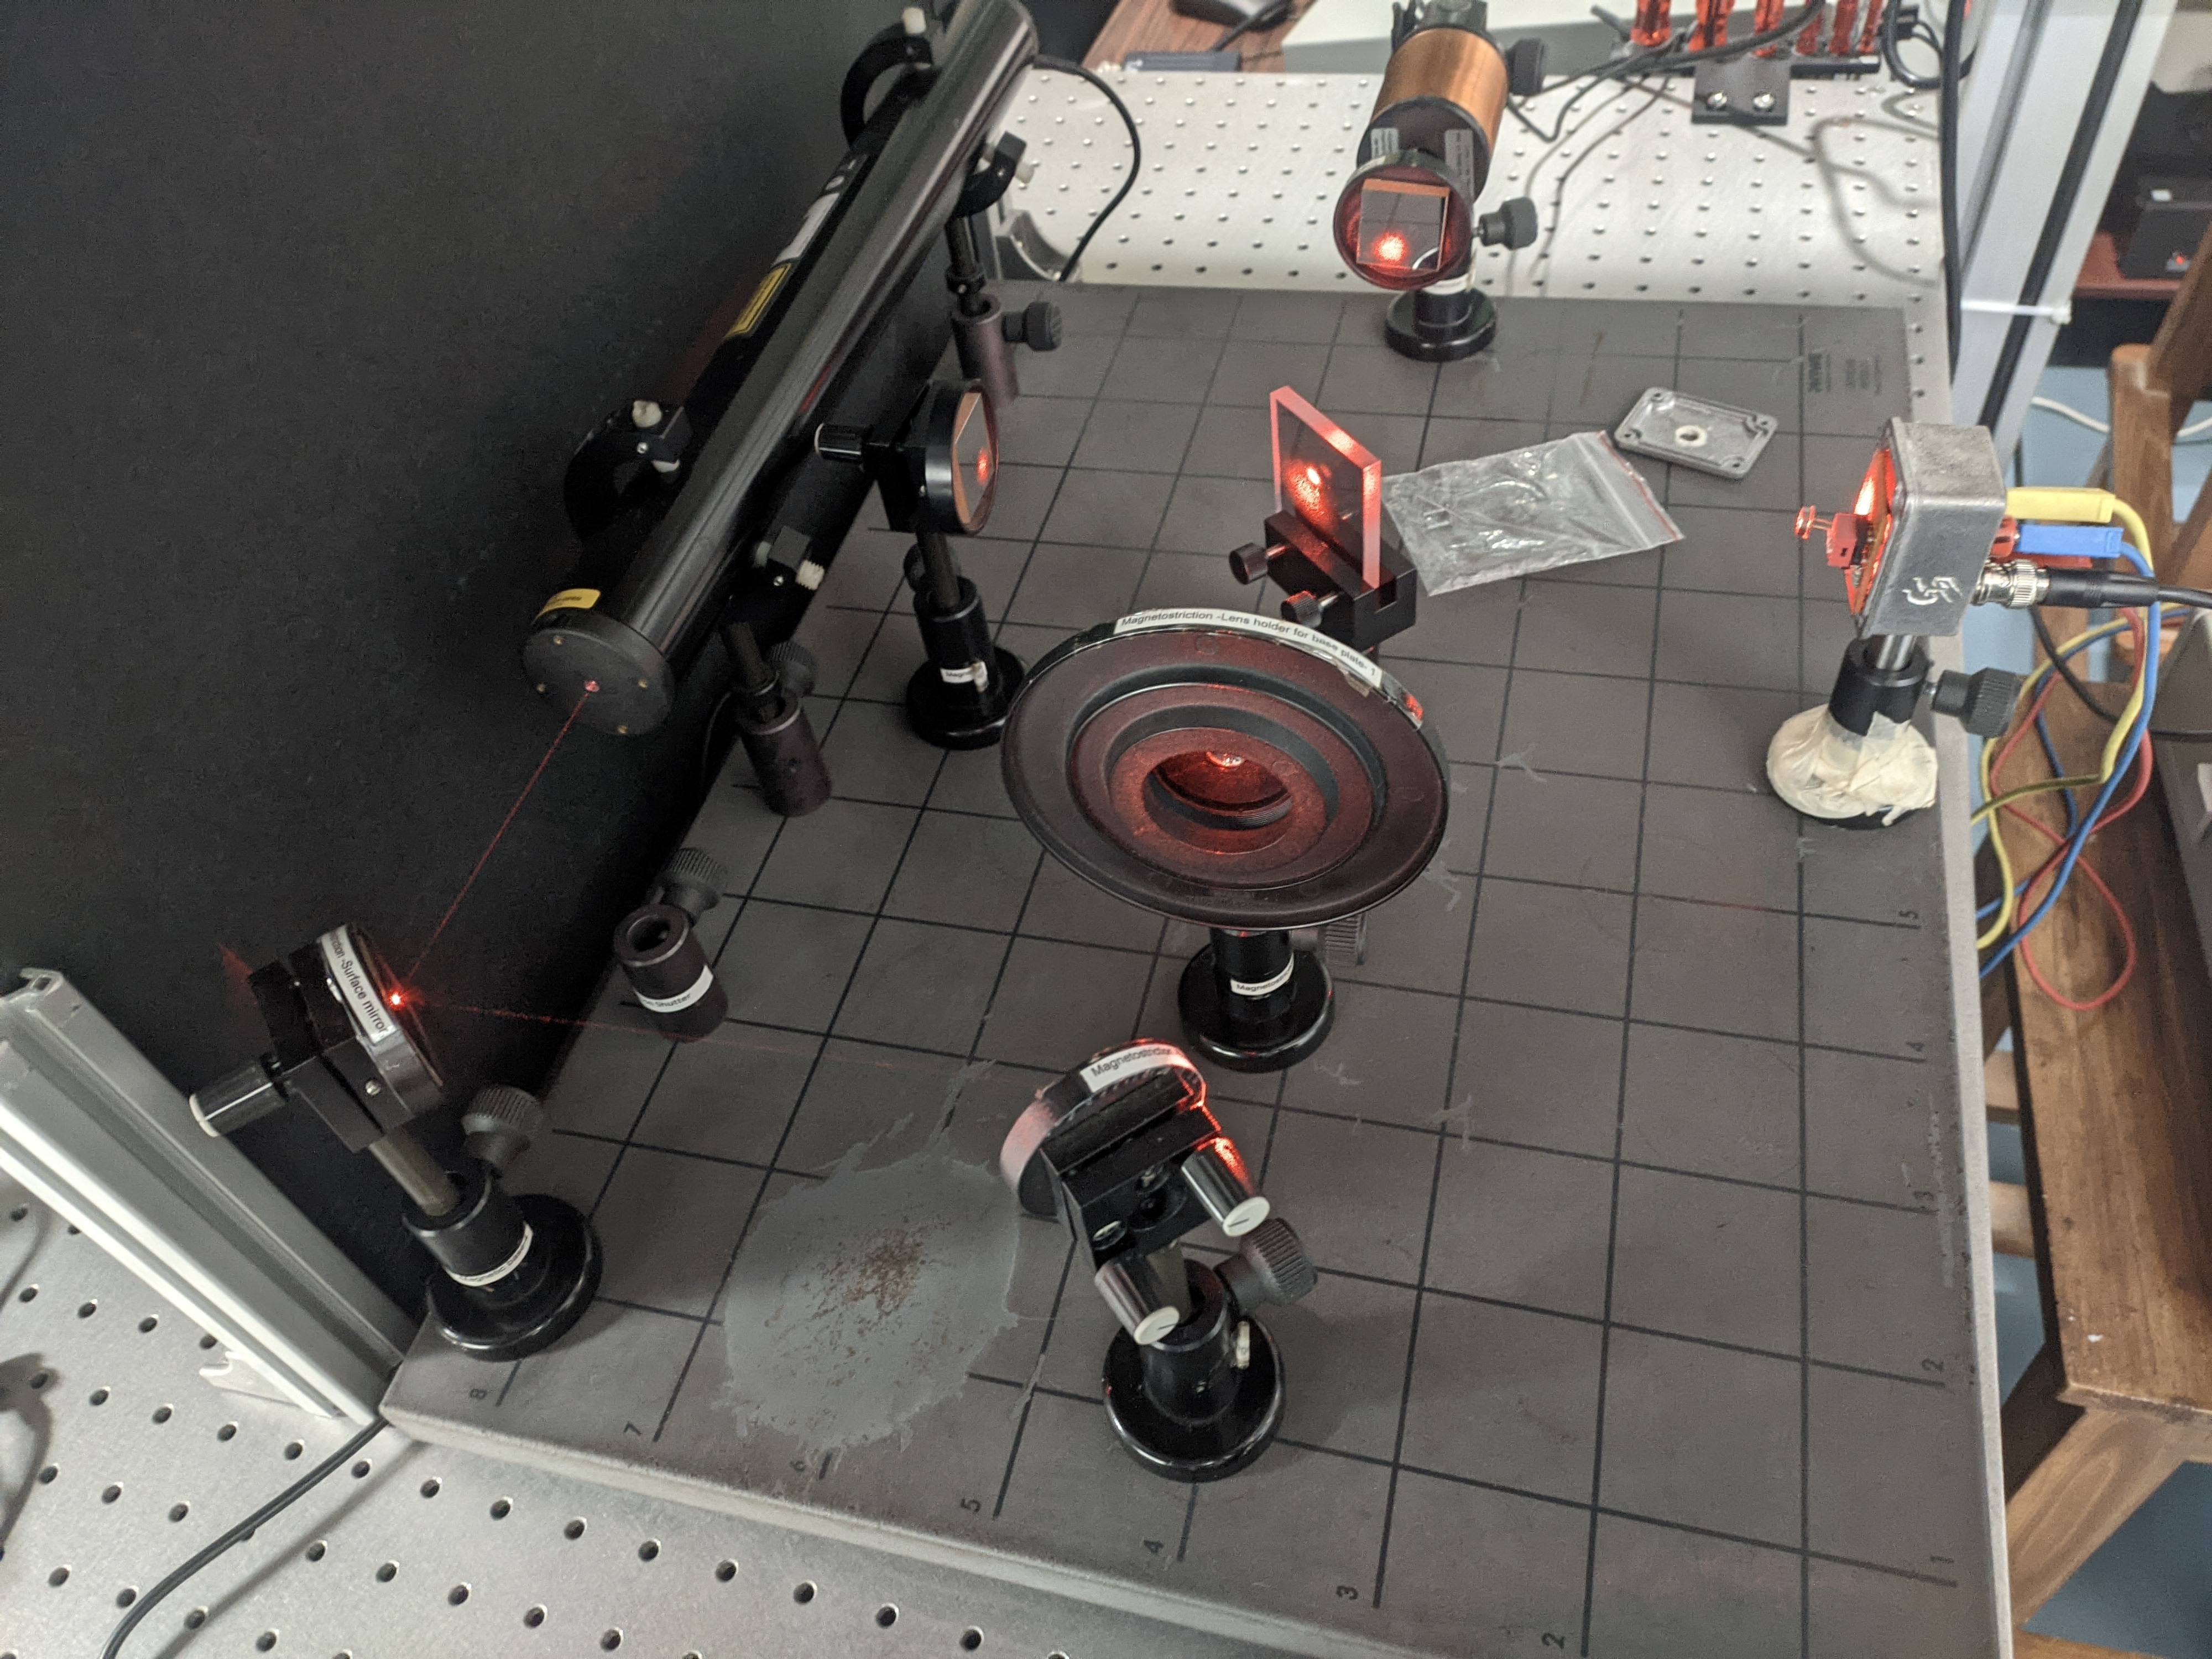
\includegraphics[width=0.7\linewidth]{SGCAM_20230117_144136325}
	\caption{Experimental set-up}
	\label{fig:sgcam20230117144136325}
\end{figure}
Here for getting more plot points we count
the bright and dark fringes which sinks in or
source out. So, in the calculations and further
discussions n will vary as 0.5, 1, 1.5, 2... Thereby
the formula gets modified to:
\begin{equation}
	\Delta l = n \dfrac{\lambda}{4}
\end{equation}

\begin{figure}
	\centering
	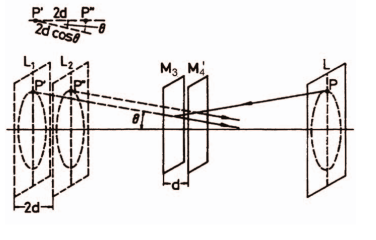
\includegraphics[width=0.7\linewidth]{mich-2}
	\caption{Formation of circular interference fringes}
	\label{fig:mich-2}
\end{figure}

\begin{figure}
	\centering
	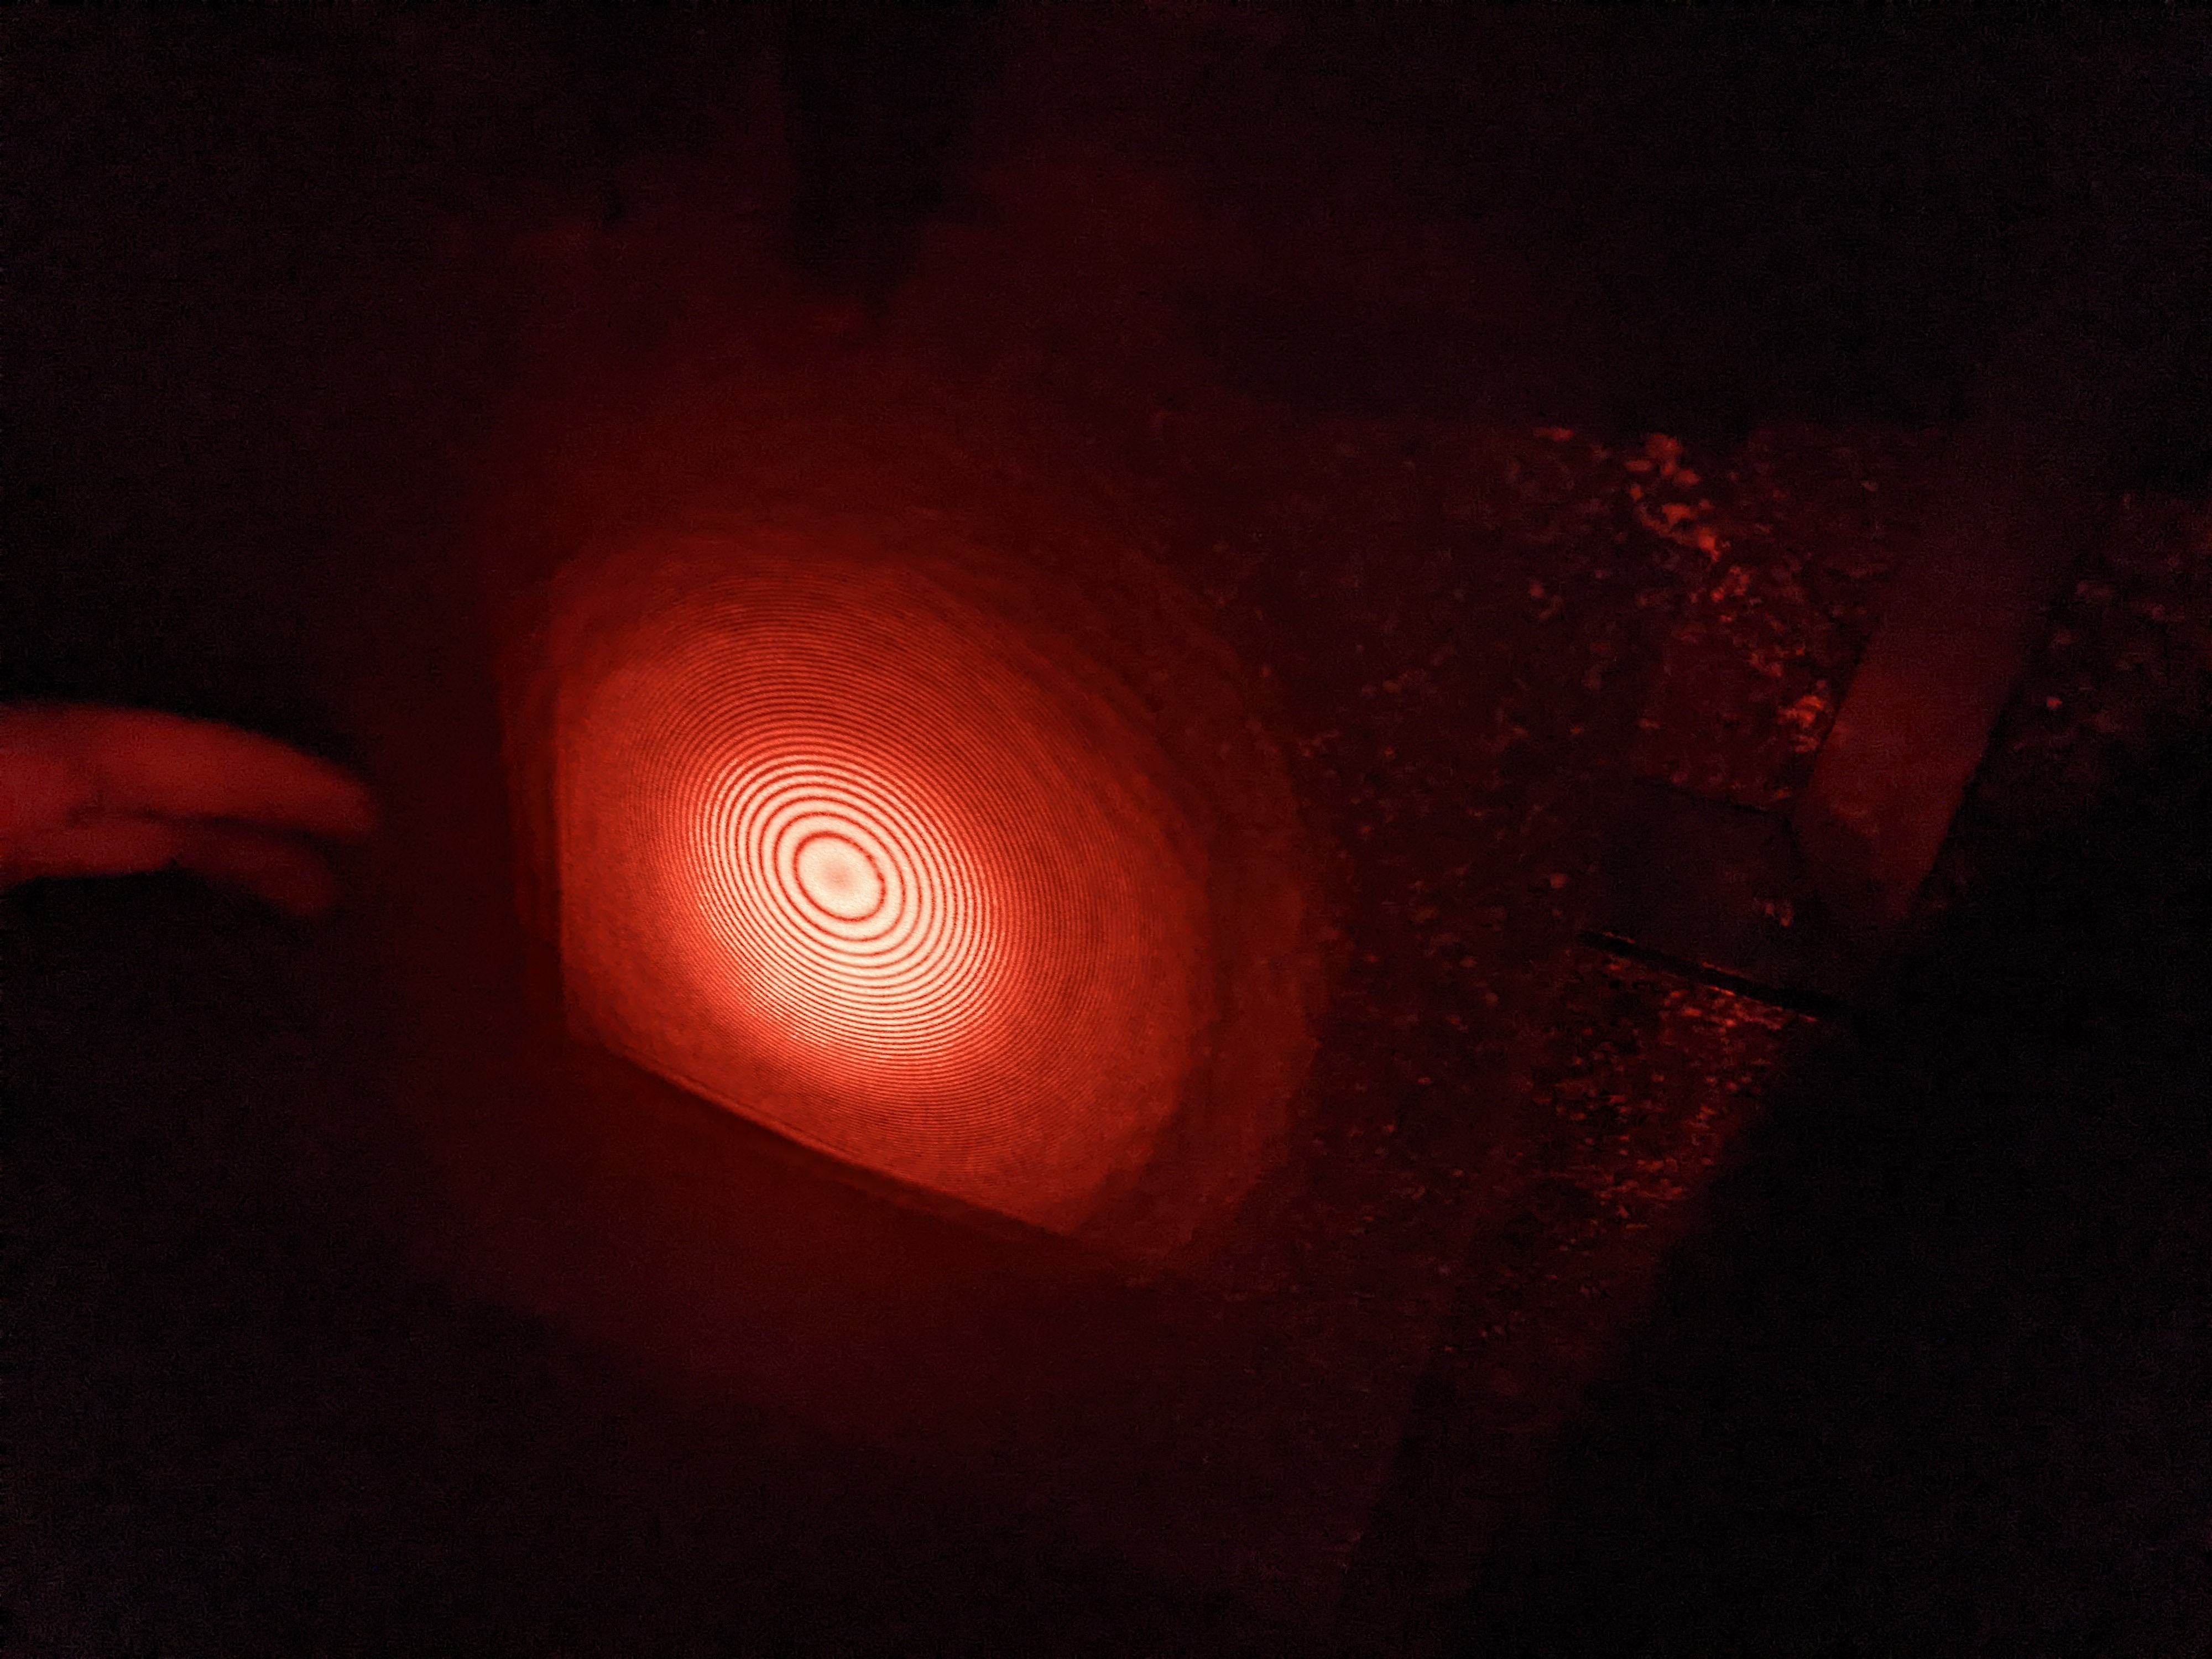
\includegraphics[width=0.7\linewidth]{SGCAM_20230117_144255387}
	\caption{Circular fringes observed on the screen after alignment.}
	\label{fig:fringes}
\end{figure}
The output of the interferometer falls on a photodetector system that measures the number of fringes that have shifted. A voltage is produced as an output from the photodetector. The output from the photodetector is then connected to a digital multimeter PPH-1503, which is connected to a PC. This PC has Labview software installed where a counting program is writtent to get the data on shifted fringes. This software is also used to regulate the current provided to the coil. The coil is also connected to the PPH-1503 to facilitate this process.


\begin{figure}[H]
	\centering
	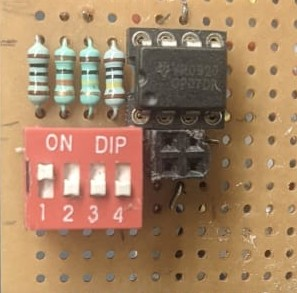
\includegraphics[width=0.5\textwidth]{circuit.jpeg}
	\caption{Detector Circuit}
	\label{fig:flow around cylinder}
\end{figure}

This entire setup is done on an optical bench which is supported by pneumatic vibration isolators. This allows us to get results which are free from noise.
\begin{figure}[H]
	\centering
	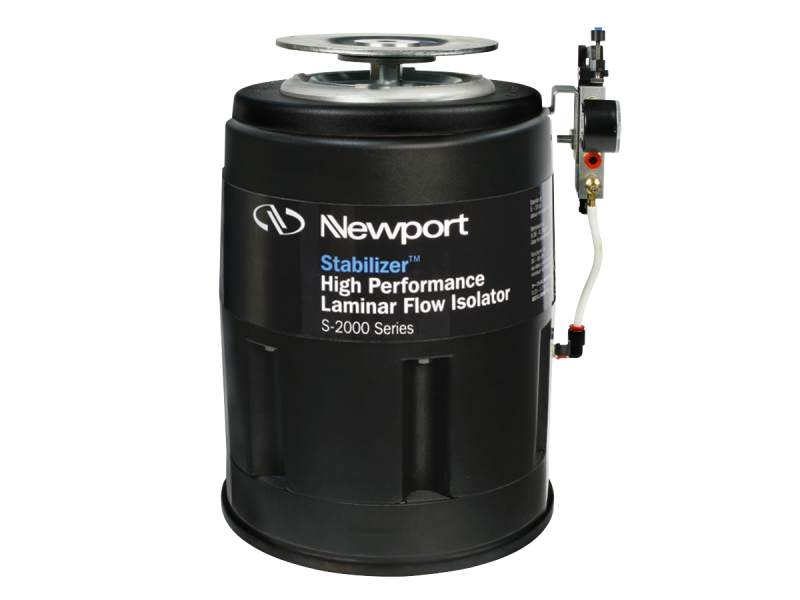
\includegraphics[width=0.5\textwidth]{newport.jpg}
	\caption{Vibration Isolator}
	\label{fig:flow around cylinder}
\end{figure}
\setcounter{equation}{0}
\setcounter{table}{0}
\setcounter{figure}{0}
%\baselineskip 24pt
